\chapter{Analysis}

In this chapter, we will discuss the decisions we made during application design and reasons behind every choice. We will define what influenced the chosen application structure. Finally, we will explain the purpose of each part of the application.

%%-----------------------------------------------------------------------------------------
%% SECTION
%%-----------------------------------------------------------------------------------------
\section{Use Case Scenarios And Requirements}

We would like to start with describing a few real life use case scenarios of our application. These will help us to get a better understanding of the issue and to define user requirements.
\begin{itemize}
    \item An entrepreneur is establishing a new bar. The new bar focuses on younger clientele. The entrepreneur already has the interior designed but has not solved the sound system yet. A classic jukebox does not match the interior design and additionally, the pursued clientele does not carry cash or change anymore.
    \item The owner of an establishment, where customers spend a lot of time waiting~(e.g. hairdressers, doctor's surgery), would like to make the waiting more pleasant by playing music. The owner has no particular knowledge about the music preference of their customers and would like to allow the customers to choose the music themselves while they wait.
    \item Peter throws a New Year's Eve party for his friends. He has a good collection of music on his computer. The music preference of his guests is varied so he would like to allow his guests to choose their songs. However, Peter has a lot of private things on his computer and he would not like to allow his guests to use his computer without his supervision nor would he like to spend the whole evening sitting at his computer instead of spending time with his guests.
\end{itemize}

\par
More formally, the user of the application (further referenced to as "spot admin") would like to let other people (further referenced to as "guests") to choose what songs are being played in the application in their "music spot". Spot admin can define what songs are currently available to choose from and has control over music playback. Guests can browse available songs on a different device (e.g. mobile application on their phones) and enqueue their ordered songs in a queue.
\par
This thesis focuses on designing and developing an application for music playback used by spot admins. The design of application for guests is not part of this thesis. Such application considers slightly different user requirements and requires a different skill set outside of the expertise of the author of this thesis. A friend of the author works on developing a mobile app for guests that integrates with our application via a common data management system available via internet. The details of the integration of the mobile app will be explained later.

%%-----------------------------------------------------------------------------------------
\subsection{User Requirements and Functionality}

Based on the previously mentioned scenarios we are now able to formulate user requirements that our applications tries to fulfill. These define the functionality that the application offers and its design. 
\begin{itemize}
    \item Playing music is the core functionality of the application. It is important to support decoding of multiple popular audio formats and outputting the audio to an audio device.
    \item A song queue is a common thing known from jukeboxes. Multiple guests may order songs simultaneously or before a previous song has finished. Ordered songs are held in a queue and played one after the other based on when they were ordered.
    \item Music playback should be continuous. Music should play even when no songs are ordered by guests. The application should select song order by itself in such situations to limit required user supervision.
    \item Another important requirement is music library. A music library stores and manages a collection of music files. A varied music library may contain thousands of music files. These music files will be offered to regular users to choose from. Users may also create playlists. Playlists allow to group music files within a music library. These can be used to offer different sets of songs on different occasions.
    \item User system is important for user authentication. Spot admins may provide a description of their music spot as part of their user account. Guests may discover music spots available close to them. It also lays the basis for potential payment system for ordered songs.
    \item Graphical user interface is necessary to allow users to easily interact with the application.
    \item The solution needs to be scalable to handle increasing number of guests within a music spot and to handle increasing size of music library. These two numbers should not limit the usability of the application.
    \item The application should be platform independent. Different use cases and users may prefer or require different platforms to run the application. Platform independence provides more potential users.
    \item Internationalization of the application is a necessity. Even within Czech Republic potential spot admins might speak different languages~(e.g. foreign owners of establishments, exchange students, minorities etc.). The application should be designed to support localization to different languages.
    \item The application should offer means of customization to accommodate a wide range of use cases.
\end{itemize}

%%-----------------------------------------------------------------------------------------
\section{Modular Application}

The range of possible use-cases of our application is wide. It can be seen earlier on the real life scenarios. Each of them have different requirements. The users would therefore appreciate the option to customize the application based on their needs. Application design should be able to accommodate these needs.
\par
One of the possible differences is the required complexity of provided services. Some users might prefer simple "Plug \& Play" type of application that is simple to set up, simple to start and the music is playing. Others might require complex audio settings and/or complex playlist creation and management tools.
\par
Additionally, our application extensively uses hardware. Whether it is speakers, which may require complex wiring in larger buildings, internet connection to communicate with mobile applications or data storage devices containing music libraries. Users might appreciate if they would not have to provide access to all of these resources on one device.
\par
The idea is to design a modular application. The application would be split into multiple separable modules. A module represents a separable process. Each module has specific role and defines unique functionality and services that it should provide. Modules communicate via network and together they provide all functionality that the application offers. They have predefined application programming interfaces that define how their services can be accessed and how to communicate with them. A module may then be implemented in multiple ways - as a stand-alone executable program or multiple modules may be combined together in one executable program. These may then run on devices owned by user or on a server.
\par
By adopting this approach it is possible to create multiple implementations of certain modules. Each implementation of module might offer different level of required functionality and services or support different platforms and devices. Users might select the most suitable implementation for them.
\par 
Additionally, modules can be separated from each other based on specific local conditions. Each of them can run on a different machine, or all on one. The only requirement is network access for communication. That should not be a limiting factor thanks to capabilities of current wireless network technologies.
\par 
Last, but not least, not all modules would have to be run by the user. There can be modules providing services to multiple users such as a shared music library server.

%%-----------------------------------------------------------------------------------------
%% SECTION
%%-----------------------------------------------------------------------------------------
\section{Definition Of Modules}

Each module should contain functionality that may be required to be separated from the rest of the application. That functionality would then be offered as services of the module. Defining too many modules might introduce unnecessary complexity. Too few modules might not provide desired flexibility. In this section we explain what is the purpose of each module and reason why it is separated from the rest of modules.

%%-----------------------------------------------------------------------------------------
\subsection{Manager Module}

The most important module from the perspective of the user is the "Manager" module. This module provides graphical user interface~(GUI) for the user and manages the flow of the application as a whole.
\par
The GUI should allow the user to manage whole application from one place. It should offer controls for controlling music playback, browsing through music library, creating and editing playlists, managing song order, editing user and music spot details etc. Services provided by other modules via their APIs are in a computer-friendly form so the GUI provides human-friendly way to access them.
\par
Usually, an application that offers frontend~(GUI) requires backend to process user input and handle business logic. In Manager module, backend communicates with other modules and deals with other things like maintaining continuous music playback and processing orders from guests. It would be possible to separate backend into another module so that multiple frontend users could access a single backend instance~(e.g. multiple waiters working with one application instance in a bar). However, backend design reflects frontend requirements and different GUI implementations would have different requirements. Therefore both frontend and backend are a part of Manager module. Splitting them into two modules would either lead to limiting capabilities of their implementations or defining a too complex interface between them. It is important to note that an implementation of this module where frontend and backend are separated is still possible.

%%-----------------------------------------------------------------------------------------
\subsection{Fileserver Module}

Fileserver module stores a music library. A music library is a source of music files for playback. It is a collection of music files that supports browsing through its contents. The module also supports distribution of music files. Additionally, it offers tools for creating and managing playlists as playlists consist of music files available within a music library.
\par
Music library is an expensive resource. It may require a considerable amount of disk storage. It might be appropriate to have this storage moved remotely (e.g. because of its physical size, safety or cooling requirements) or in a cloud storage. Furthermore, music is subject to copyrights. Acquiring a large amount of music files might get expensive. Therefore it might be useful to use a public Fileserver instead which offers its service for a monthly fee similarly to music streaming services such as Spotify. These are the two main reason why Fileserver is a separate module.
\par
A music file is a file that contains audio data (raw or encoded) and usually also metadata about the content such as title, author or album name. It is important to realize that these metadata are displayed to users~(spot admins or guests) when they browse through music library. The actual audio data are important only for music playback, which is the only time when an entire music file is transferred.

%%-----------------------------------------------------------------------------------------
\subsection{Player Module}

Next module is "Player" module. Its role is to play music. It is supplied with music files. All music files are encoded using a specific codec\footnote{A typical digital audio coder, or codec for encoder-decoder, is a device that takes analogue audio signals as input and transforms them temporarily into a convenient digital representation. This transformation process takes place in the encoder stage of the coder. Once we have the signal represented as a series of numbers then we can store it, process it, or transmit it. At some point, we would like to be able to listen again to the sound. To do so we need to transform the signal from its digital representation back to an analogue signal so that the human ear can detect and enjoy it. This inverse transformation from digital back to analogue takes place in the decoder stage of the coder~\citep{IntroToDigitalAudio}.}. Player module provides tools for decoding these music files utilising multiple popular audio codecs to produce data that can be sent to connected audio device to reproduce the audio.
\par
It is important to note that this module does not decide what songs are played. Its role is to play songs that are given to it as it has no knowledge of currently available songs in music spot. As it was mentioned earlier, maintaining continuous music playback and subsequently deciding the song order is handled by Manager module.
\par
Additionally, this module provides remote playback control~(e.g. play, pause, volume settings etc.). The reasons that playback can be controlled remotely are the same reasons that Player is a separate module: it is possible to give control to multiple users~(e.g. waiters in a bar) and it is possible to put the device~(e.g. a miniature PC) running this module to the most suitable location. As we mentioned earlier, in larger buildings the speakers may require complex wiring and this wiring does not have to lead to the device from which the player is controlled.

%%-----------------------------------------------------------------------------------------
\subsection{Data Management Module}

Data Management module is an important module that connects spot admins using our application with guests using mobile application. It provides services used by both groups of users as well as handles interaction between them.
\par
This module provides user authentication and user system. User system stores user preferences and settings. One shared user system is sufficient for both users and regular users. One user account can then be used to host a music spot or as a guest.
\par
Each user can own a music spot. A music spot is a place where music is played from our application. Each music spot can add its name and description. It has a list of available songs~(music file metadata) that can be ordered. Ordered songs are then added to its queue. Guests may browse available music spots and order songs when they enter them.
\par
This module therefore also stores music spot data - its basic information such as name or description, list of available songs and song queue.
\par
User authentication and music spot data should be accessible from anywhere on the internet so all users can login to their accounts and guests can discover nearby music spots wherever they are. This requirement leads to creating only one global instance and implementation of this module. There are pros and cons of such decision:
\paragraph{Pros}
\begin{itemize}
\item Users do not need to run their own instance. This module works as a server so users do not need to set up their own.
\item Guests can discover nearby music spots based on their location.
\item It is not required to provide network access to visiting guests, they can browse available songs and make orders using any internet connection~(e.g. wi-fi, cellular data etc.).
\end{itemize}

\paragraph{Cons}
\begin{itemize}
\item Application for guests has to ensure that songs can be ordered only by people present in music spot~(e.g. by location, scanning specific QR code...).
\item Running costs for operating the global instance. They can be covered by donations, fee for running a music spot or share of the revenue from sold songs in a music spot.
\end{itemize}
\par
The design of Data Management module is the reason it is separated from the rest of the application - it is not run by any of the users but all users utilise its services.

%%-----------------------------------------------------------------------------------------
\subsection{Guest Application Module}

This module is used by guests. It allows them to discover available music spots at their location and when they enter one, they can browse available songs and order them if they wish so.
\par
As we mentioned earlier, application for guests is not part of the thesis. It is developed by a friend of the author of the thesis.
\par
Even though this module can be implemented in multiple ways, we find a mobile application to be the most suitable approach. A smartphone is a common device owned by many people nowadays and mobile applications are a familiar way to interact with the surrounding digital world. However, other implementations are feasible as long as they are able to consume services provided by Data Management module.

%%-----------------------------------------------------------------------------------------
%% SECTION
%%-----------------------------------------------------------------------------------------
\section{Communication Among Modules}

Before we dive into details about each module, it would be useful to take a look at the communication among modules as it influences their designs. Modules define an application programming interface~(API) that defines how to communicate with them and allows other modules to use their services. The design of each API then depends on the content~(services that it provides) and modules that use it. In this section we will focus on that.
\par
Manager module requires no API. It provides GUI and handles business logic and no other module needs to access these services. Instead, Manager module utilizes APIs of other modules to gather data displayed in GUI and manage the flow of the application.
\par
The API of Fileserver module allows other modules to access its music library. Manager module uses this API to browse through music library and manage playlists. Player module accesses music files that it decodes to play music. Data Management module stores the list of currently available songs in music spot. However, this list is edited and selected in Manager module. Since it already has the required data~(or at least knows how to access them), Manager module can upload the list of currently available songs to Data Management module via its API. This solution removes the need to establish a connection between Fileserver and Data Management module. Fileserver module does not use API of any other module.
\par
The API of Player module provides control over music playback. That includes also order of songs besides commands like play or pause. These services are utilized by Manager module, where playback control commands are sent in response to user interaction and, as mentioned earlier, the order of songs is decided by Manager module and sent to Player module. Player module uses API of Fileserver module to get music files for decoding.
\par
Lastly, the API of Data Management module provides user authentication and access to music spot data to both Manager and Guest Application modules. Manager module publishes a list of available songs when it is ready for playback and checks queue for orders. Guest Application module displays the list of available songs and adds orders to queue. This module does not use API of any other module.
\par
Figure \ref{fig02:communicationAmongModules} shows the above-mentioned relationship among modules. An arrow leads from module which API is used to module that uses the API and describes what services are used.

\begin{figure}[ht]\centering
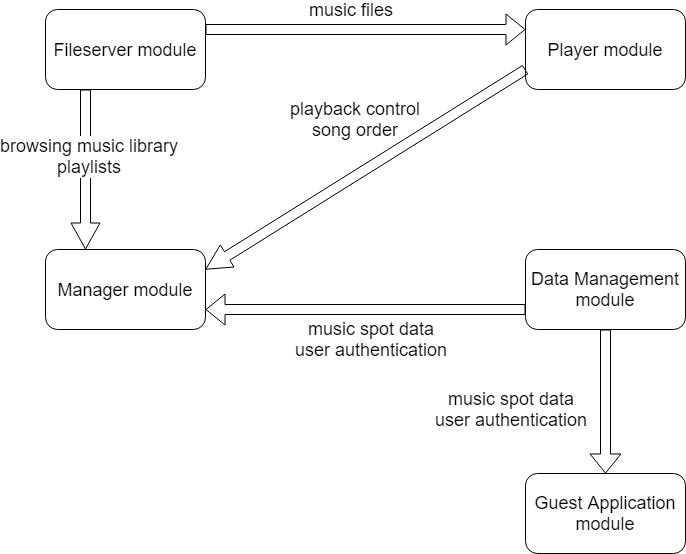
\includegraphics[width=1.0\textwidth]{img/CommunicationGraph2}
\caption{Communication among modules}
\label{fig02:communicationAmongModules}
\end{figure}

%%-----------------------------------------------------------------------------------------
%% SECTION
%%-----------------------------------------------------------------------------------------
\section {Manager Module}

Manager module provides graphical user interface~(GUI) that allows spot admins to interact with the application. This GUI is used to control most of the application functionality. It is expected to provide these controls:
\begin{itemize}
    \item User login and registration controls.
    \item Controls for selecting/connecting to Player and Fileserver modules.
    \item Controls for browsing through music library.
    \item Controls to create and manage playlists. Playlists consist of songs within a music library.
    \item Music player controls.
    \item Controls for editing music spot details.
    \item Controls for managing order of songs and queue.
    \item Application and user settings.
\end{itemize}

\par
There are multiple ways to create a GUI - classic desktop applications, web applications and mobile application. Since Manager module utilizes APIs of all of the other modules, these APIs should use technologies that restrict none of the mentioned ways if possible.
\par
Manager module is also responsible for the flow of the application. There are multiple tasks that it needs to handle. When the spot admin wants to begin music playback, module has to publish the list of songs that admin selected to Data Management module so guests can see it. It manages what songs are played by Player module by passing it either song orders from guests or selecting a random song when there are no orders. It gathers song orders from Data Management module.

















